\documentclass{standalone}
\usepackage{tikz}
\usepackage{tikz-qtree}
\usepackage[makeroom]{cancel}
\usetikzlibrary{fit}

% ОПИСАНИЕ: модификация старого алгоритма tree overlap чтобы покрывать все деревья 
\begin{document} 
	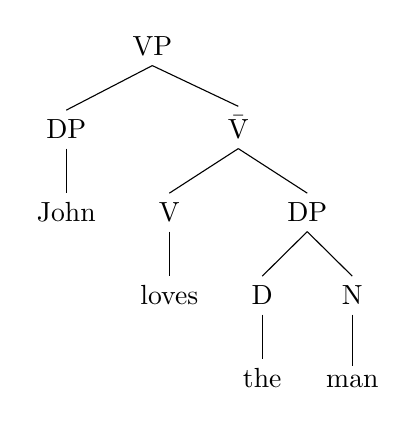
\begin{tikzpicture}[sibling distance=9.5pt]
	    \Tree [.VP [.DP John ] [.{\=V} [.V loves ] [.DP [.D the ] [.N man ] ]]]
	\end{tikzpicture}
\end{document} 